\chapter{Estado del arte}
En este capítulo se hablará sobre el contexto en el que se enmarca este proyecto.

En primer lugar, se hará una breve explicación de como las herramientas open-source ayudan a agilizar el desarrollo y la funcionalidad en una red de telecomunicaciones.

Por último, se hace especial mención a los dos paradigmas que motivan este proyecto: SDN y NFV.

\section{Herramientas Open-Source en redes de telecomunicación}

Una red de telecomunicación es un conjunto de medios, tecnologías y protocolos que tienen como finalidad el intercambio de información entre diferentes usuarios.

Así mismo, 


\section{SDN}
\label{sec:sdn}

\begin{figure}[!ht]
	\centering
	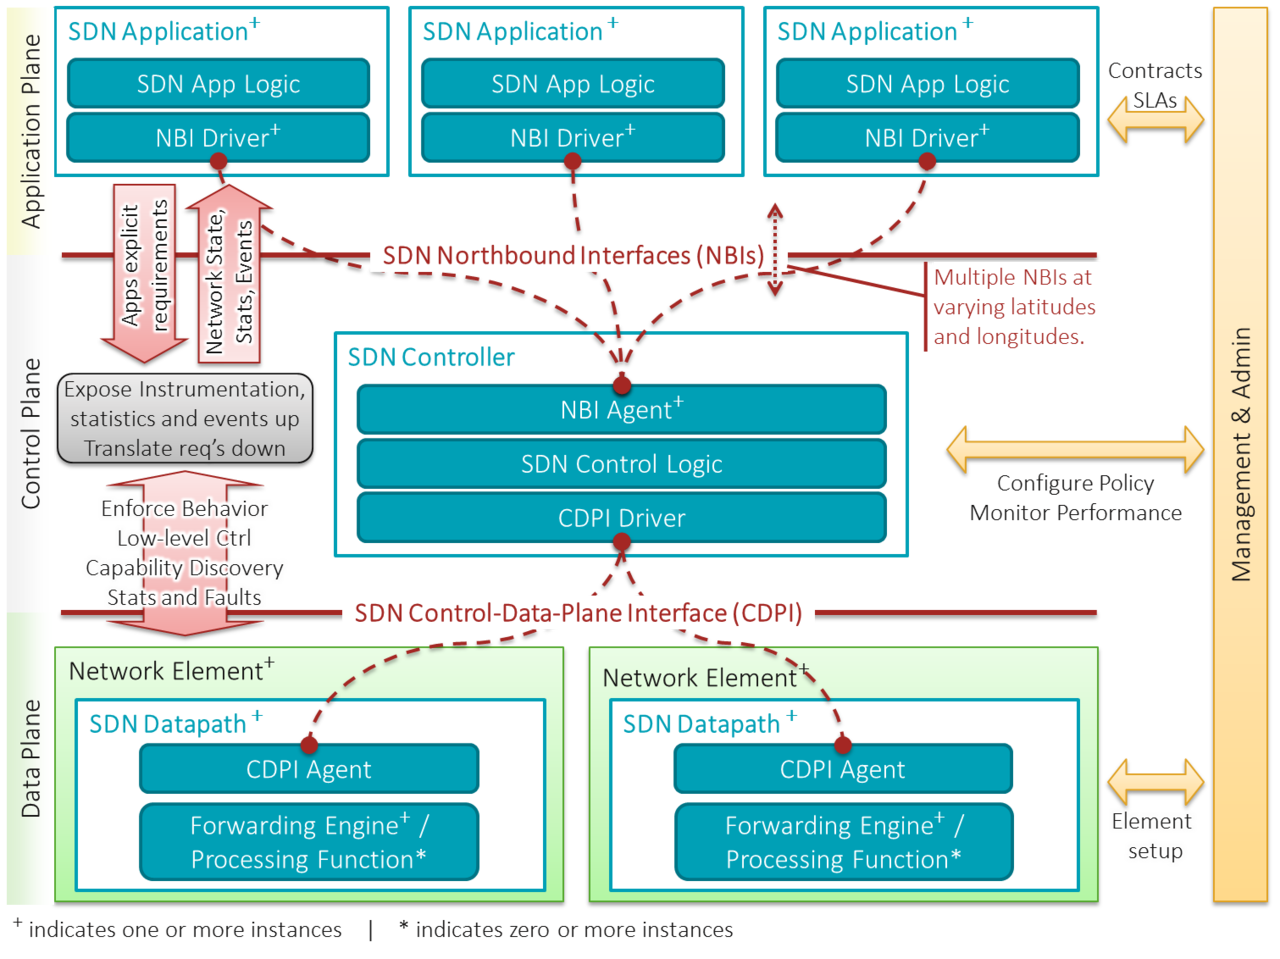
\includegraphics[width=0.75\linewidth]{imagenes/arquitectura_sdn}
	\caption{Arquitectura SDN}
	\label{fig:arquitecturasdn}
\end{figure}


\subsection{OpenFlow}
\label{subsec:openflow}

\section{NFV}
\label{sec:nfv}


\cleardoublepage